\section{Back-end}
        \subsection{Giới thiệu kiến trúc Microservices}
        Trước khi Microservices xuất hiện, các ứng dụng thường phát triển theo mô hình Monolithic architecture (Kiến trúc một khối). Có nghĩa là tất cả các module (view, business, database) đều được gộp trong một project, một ứng dụng được phát triển theo mô hình kiến trúc một khối thường được phân chia làm nhiều module. Nhưng khi được đóng gói và cài đặt sẽ thành một khối (monolithic). Lợi ích của mô hình kiến trúc một khối đó là dễ dàng phát triển và triển khai. Nhưng bên cạnh đó nó cũng có nhiều hạn chế ví dụ như khó khăn trong việc bảo trì, tính linh hoạt và khả năng mở rộng kém, đặc biệt với những ứng dụng doanh nghiệp có quy mô lớn. Đó chính là lí do ra đời của kiến trúc Microservices. Với lý do đó nhóm sẽ chọn phát triển hệ thống theo kiến trúc Microservices.
        \begin{itemize}
            \item Những đặc điểm của Microservices
            \begin{itemize}
                \item \textbf{Decoupling} - Các service trong một hệ thống phần lớn được tách rời. Vì vậy, toàn bộ ứng dụng có thể dễ dàng được xây dựng, thay đổi và thu nhỏ.
                \item \textbf{Componentization} - Microservices được coi là các thành phần độc lập có thể dễ dàng thay thế và nâng cấp.
                \item \textbf{Business Capabilities} - Mỗi một thành phần trong kiến trúc microservice rất đơn giản và tập trung vào một nhiệm vụ duy nhất.
                \item \textbf{Autonomy} - Các lập trình viên hay các nhóm có thể làm việc độc lập với nhau trong quá trình phát triển.
                \item \textbf{Continous Delivery} - Cho phép phát hành phần mềm thường xuyên, liên tục.
                \item \textbf{Decentralized Governance} - Không có mẫu chuẩn hóa hoặc bất kỳ mẫu công nghệ nào. Được tự do lựa chọn các công cụ hữu ích tốt nhất để có thể giải quyết vấn đề.
                \item \textbf{Agility} - Microservice hỗ trợ phát triển theo mô hình Agile.
            \end{itemize}
            \item Ưu điểm\\\\
            Kiến trúc Microservices được sinh ra để khắc phục những hạn chế của kiến trúc một khối. Kiến trúc Microservices giúp đơn giản hóa hệ thống, chia nhỏ hệ thống ra làm nhiều service nhỏ lẽ dễ dàng quản lý và triển khai từng phần so với kiến trúc nguyên khối. Phân tách rõ ràng giữa các service nhỏ. Cho phép việc mỗi service được phát triển độc lập. Cũng như cho phép lập trình viên có thể tự do chọn lựa công nghệ và ngôn ngữ cho mỗi service mình phát triển. Mỗi service có thể được triển khai một cách độc lập (VD: Mỗi service có thể được đóng gói vào một docker container độc lập, giúp giảm tối đa thời gian deploy). Nó cũng cho phép mỗi service có thể được mở rộng một cách độc lập với nhau. Việc mở rộng có thể được thực hiện dễ dàng bằng cách tăng số instance cho mỗi service rồi phân tải bằng load balancer.
            \begin{itemize}
                \item \textbf{Independent Development} - Tất cả các service có thể được phát triển dễ dàng dựa trên chức năng cá nhân của từng service. Có thể chia nhỏ để phát triển độc lập.
                \item \textbf{Independent Deployment} - Có thể được triển khai riêng lẻ trong bất kỳ ứng dụng nào.
                \item \textbf{Fault Isolation} - Khi một service của ứng dụng không hoạt động, hệ thống vẫn tiếp tục hoạt động.
                \item \textbf{Mixed Technology Stack} - Các ngôn ngữ và công nghệ khác nhau có thể được sử dụng để xây dựng các service khác nhau của cùng một ứng dụng.
            \end{itemize}
            \item Nhược điểm
            \begin{itemize}
                \item Kiến trúc Microservices đang là một xu hướng, nhưng nó cũng có nhược điểm của nó. Microservice khuyến khích làm nhỏ gọn các service, nhưng khi chia nhỏ sẽ dẫn đến những thứ vụn vặt, khó kiểm soát. Hơn nữa chính từ đặc tính phân tán khiến cho các lập trình viên phải lựa chọn cách thức giao tiếp phù hợp khi xử lí request giữa các service.
                \item Hơn nữa việc quản lí nhiều database, và transaction giữa các service trong một hệ thống phân tán cũng là một khó khăn không nhỏ. Hay khi thực hiện test một service, bạn cũng cần test các service có liên quan.
                \item Triển khai microservice cũng sẽ phức tạp hơn so với ứng dụng kiến trúc một khối, cần sự phối hợp giữa nhiều service, điều này không đơn giản như việc triển khai WAR trong một ứng dụng kiến trúc một khối.
            \end{itemize}
            \item Với những ưu điểm và nhược điểm đã được nói ở trên nên nhóm đã quyết định sử dụng kiến trúc Microservices để xây dựng hệ thống của nhóm.
        \end{itemize}
		\subsection{Kiến trúc Microservicces}
		Các thành phần chính dự kiến xây dựng hệ thống trong Microservices
		\begin{itemize}
		    \item \textbf{Edge Server} - Để đưa các API services ra bên ngoài và để ngăn chặn truy cập trái phép vào các microservices nội bộ, chúng ta cần một edge server nơi tất cả request bên ngoài đi qua. Một edge server có thể tái sử dụng khả năng định tuyến động và cân bằng tải dựa trên service discovery được mô tả ở trên. Edge server sẽ hoạt động như một proxy ngược chủ động mà không cần cập nhật thủ công khi hệ thống nội bộ thay đổi.
		    \item \textbf{Dynamic Routing and Load Balancer} - Với chức năng service discovery, các thành phần định tuyến có thể sử dụng discovery API để tra cứu nơi mà microservice được yêu cầu được triển khai và các thành phần cân bằng tải có thể quyết định định tuyến yêu cầu tới instance nào nếu nhiều instance được triển khai cho một service được yêu cầu.
		    \item \textbf{Service Discovery} - Thay vì theo dõi thủ công những microservices nào được triển khai hiện tại và trên máy chủ và cổng nào, chúng ta cần chức năng Service Discovery cho phép microservices tự đăng ký khi khởi động thông qua API.
		    \item \textbf{Circuit Breaker} - Để tránh chuỗi sự cố, cần phải áp dụng Circuit Breaker pattern. Đây là một pattern dùng để ngắt một quá trình xử lý khi hệ thống gặp sự cố, để đảm bảo số lượng message bị lỗi không tăng cao, làm cho việc khắc phục trở nên khó khăn, cũng như có thể làm cho hệ thống bị xụp đổ hàng loạt do ảnh hưởng lẫn nhau.
		    \item \textbf{Monitoring} - Vì đã có circuit breakers, chúng ta có thể bắt đầu theo dõi trạng thái của chúng và thu thập số liệu thống kê thời gian chạy từ chúng để có được một bức tranh về tình trạng sức khỏe của hệ thống.
	        \item \textbf{Secure API} - Để bảo vệ các API services được expose ra bên ngoài sử dụng OAuth 2.0, quy trình của OAuth 2.0 có thể như sau:
	        \begin{itemize}
	            \item Một component mới có thể đóng vai trò như một máy chủ ủy quyền (OAuth Authorization Server)
	            \item Các API services sẽ đóng vai trò như các máy chủ tài nguyên (OAuth Resource Server)
	            \item Các Client bên ngoài gọi đến API services với tư cách là OAuth Clients
	            \item Edge server sẽ làm việc như một OAuth Token Relay: nó sẽ hoạt động như một OAuth Resource Serve, Nó sẽ chuyển các OAuth Access Tokens có trong request bên ngoài đến các API services
	        \end{itemize}
	        \item \textbf{Central Configuration Server.} - Thay vì cấu hình cục bộ cho mỗi đơn vị triển khai (tức là microservice), chúng ta cần quản lý cấu hình tập trung. Chúng ta cũng cần một configuration API để các microservices có thể sử dụng để lấy thông tin cấu hình.
	        \item \textbf{Centralized Log Analysis} - Để có thể theo dõi messages và phát hiện khi chúng bị kẹt (stuck), chúng ta cần một chức năng phân tích log tập trung có khả năng tiếp cận với máy chủ và thu thập các tệp log mà mỗi services microservice tạo ra. Chức năng phân tích log lưu trữ thông tin log này trong cơ sở dữ liệu trung tâm và cung cấp khả năng tìm kiếm và dashboard. Lưu ý : Để có thể tìm thấy các messages liên quan, điều quan trọng là tất cả các microservices phải sử dụng id đồng nhất trong các log message.
		\end{itemize}
	
		\begin{figure}[H]
			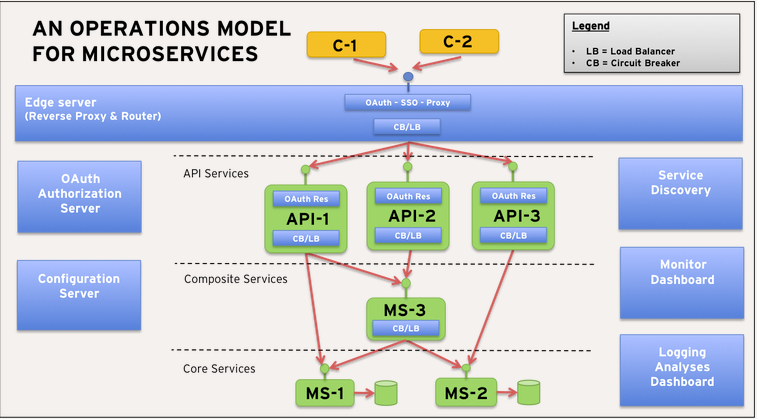
\includegraphics[width=0.8\textwidth]{Images/model-microservice.png}
			\centering
			\linebreak
			\caption{Mô hình Microservices}
		\end{figure}		

		\subsection{Công nghệ tổng quan}
		Công nghệ nền tảng dự kiến sử dụng của nhóm: SPRING BOOT, SPRING CLOUD VÀ SPRING SECURITY
		\begin{itemize}
		    \item \textbf{Spring Boot} là một dự án nổi bật trong hệ sinh thái Spring Framework. Nếu như trước đây, công đoạn khởi tạo một dự án Spring khá vất vả từ việc khai báo các dependency trong file pom.xml cho đến cấu hình bằng XML hoặc annotation phức tạp, thì giờ đây với Spring Boot, chúng ta có thể tạo các ứng dụng Spring một cách nhanh chóng và cấu hình cũng đơn giản hơn.
		    \item \textbf{Spring Cloud} là nền tảng khá mới mẻ trong gia đình Spring.io dùng để xây dựng microservice một cách nhanh chóng. Spring Cloud cung cấp các công cụ cho các lập trình viên để nhanh chóng xây dựng một số common patterns trong các hệ thống phân tán (e.g. configuration management, service discovery, circuit breakers, intelligent routing, micro-proxy, control bus, one-time tokens, global locks, leadership election, distributed sessions, cluster state). Chúng sẽ hoạt động tốt trong bất kỳ môi trường phân tán nào, bao gồm máy tính xách tay của chính lập trình viên, các data center hoặc trên cloud.
		    \item \textbf{Spring Security} là một trong những core feature quan trọng của Spring Framework, nó giúp chúng ta phân quyền và xác thực người dùng trước khi cho phép họ truy cập vào các tài nguyên của chúng ta. 
		\end{itemize}
		Công nghệ sử dụng cho Secure API
		\begin{itemize}
		    \item \textbf{Json Web Token(JWT)} - Là 1 tiêu chuẩn mở (RFC 7519) định nghĩa cách thức truyền tin an toàn giữa các thành viên bằng 1 đối tượng JSON. Thông tin này có thể được xác thực và đánh dấu tin cậy nhờ nó có chứa chữ ký số (digital signature). Phần chữ ký của JWT sẽ được mã hóa lại bằng HMAC hoặc RSA. Sử dụng JWT là cách tốt để áp dụng cơ chế bảo mật đối với các dịch vụ API RESTful mà có thể được sử dụng để truy cập vào cơ sở dữ liệu.
		\end{itemize}
        \subsection{Kiến trúc RESTful API}
		    
		    RESTful API là một tiêu chuẩn dùng trong việc thiết kế các API cho ứng dụng web để quản lý tài nguyên. RESTful là một trong những kiểu thiết kế API được sử dụng phổ biến ngày nay để cho các ứng dụng (web, mobile, web service...) khác nhau có thể giao tiếp với nhau.\\
		    
		    Khi làm việc với server sẽ gồm 4 hoạt động thiết yếu đó là: lấy dữ liệu, tạo mới, cập nhật, xóa dữ liệu.\\
		    
		    REST hoạt động chủ yếu dựa vào giao thức HTTP. Mỗi trong 4 hoạt động cơ bản trên sẽ sử dụng những phương thức HTTP riêng (HTTP method):
		    
		    \begin{itemize}
		        \item POST (CREATE) : Tạo mới một tài nguyên.
		        \item GET (READ) : Trả về một tài nguyên hoặc một danh sách tài nguyên.
		        \item PUT (UPDATE) : Cập nhật, thay thế thông tin cho tài nguyên.
		        \item DELETE (DELETE) : Xóa một tài nguyên.
		    \end{itemize}
		    REST là một kiến trúc thống nhất giúp thiết kế các website để có thể dễ dàng quản lý các tài nguyên. Nó không phải là một quy luật buộc phải tuân theo mà đơn giản là một kiến trúc được đề xuất ra và kiến trúc này hiện đang được sử dụng rất phổ biến vì tính đơn giản, dễ hiểu và rất ưu việt của nó. Với các ứng dụng web được thiết kế sử dụng RESTful, có thể dễ dàng biết được URL và HTTP method để quản lý một tài nguyên.
		    
		    \begin{figure}[H]   			
		    	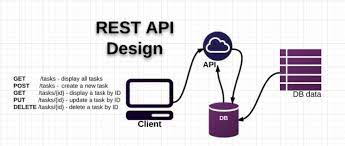
\includegraphics[width=0.8\textwidth]{Images/restful.jpeg}
		    	\centering
		    	\linebreak
		    	\caption{RESTFul API}
		    \end{figure}
		    
		    \textbf{Ưu điểm}
		  
	        \begin{itemize}
	            \item REST cũng có ưu điểm khi sử dụng giao thức stateless (không trạng thái). Hệ thống này không sử dụng session, cookie, không cần biết những thông tin đó trong mỗi lần request đến máy chủ ngoài. Điều này giúp REST giảm tải cho máy chủ ngoài, nâng cao hiệu suất làm việc.
	            \item Tính khả biến: với các hệ thống cần thay đổi các tài nguyên liên tục, sử dụng REST với việc tạo request đơn giản sẽ giúp mọi chuyện trở nên đơn giản hơn.
	            \item Tính mở rộng: các hệ thống REST có khả năng mở rộng rất cao nhờ sự tách biệt giữa các thành phần và các quy ước giao tiếp được quy định sẵn.
	            \item Tính linh hoạt: việc chuẩn hoá interface giúp hệ thống trở nên linh hoạt hơn, có thể sử dụng cho cho nhiều nền tảng khác nhau, mobile, web,...
	            \item Trong sáng: trong giao tiếp giữa các thành phần, các request trở nên rất rõ ràng, dễ hiểu.
	        \end{itemize}
	        
		    \textbf{Nhược điểm}
		    
	        \begin{itemize}
	            \item REST chỉ hoạt động trên các giao thức HTTP.
	        \end{itemize}
	 
            \subsection{MySQL}
            
            MySQL là hệ quản trị cơ sở dữ liệu tự do nguồn mở phổ biến nhất thế giới và được các nhà phát triển rất ưa chuộng trong quá trình phát triển ứng dụng. Vì MySQL là cơ sở dữ liệu tốc độ cao, ổn định và dễ sử dụng, có tính khả chuyển, hoạt động trên nhiều hệ điều hành cung cấp một hệ thống lớn các hàm tiện ích rất mạnh. Với tốc độ và tính bảo mật cao, MySQL rất thích hợp cho các ứng dụng có truy cập cơ sở dữ liệu trên internet.
            
            \begin{figure}[H]   			
\includegraphics[width=0.8\textwidth]{Images/mysqlintro.png}
            	\centering
            	\linebreak
            	\caption{Mysql}
            \end{figure}
            
            \textbf{Ưu điểm}
            
            \begin{itemize}
                \item \textbf{Dễ sử dụng}: MySQL là cơ sở dữ liệu tốc độ cao, ổn định, dễ sử dụng và hoạt động trên nhiều hệ điều hành.
                \item \textbf{Độ bảo mật cao}:  MySQL rất thích hợp cho các ứng dụng có truy cập cơ sở dữ liệu trên Internet khi sở hữu nhiều nhiều tính năng bảo mật thậm chí là ở cấp cao.
                \item \textbf{Đa tính năng}: MySQL hỗ trợ rất nhiều chức năng SQL được mong chờ từ một hệ quản trị cơ sở dữ liệu quan hệ cả trực tiếp lẫn gián tiếp.
                \item \textbf{Khả năng mở rộng và mạnh mẽ}: MySQL có thể xử lý rất nhiều dữ liệu và hơn thế nữa nó có thể được mở rộng nếu cần thiết.
            \end{itemize}
            
            \textbf{Nhược điểm}
            
            \begin{itemize}
                \item \textbf{Khả năng scale rất khó và tốn chi phí}: Nếu bản ghi lớn dần lên thì việc truy xuất dữ liệu là khá khó khăn, khi đó chúng ta sẽ phải áp dụng nhiều biện pháp để tăng tốc độ truy xuất dữ liệu như là chia tải database này ra nhiều server.	
            \end{itemize}	
            \subsection{Cassandra}
            
            Ngày nay, các dịch vụ trên Internet phải xử lí khối lượng dữ liệu rất lớn. Hầu hết dữ liệu sẽ được lưu trữ phân tán trên nhiều máy chủ khác nhau. Vì vậy, các hệ quản trị cơ sở dữ liệu quan hệ (RDBMS) tỏ ra không còn phù hợp với các dịch vụ như thế này nữa. Người ta bắt đầu nghĩ tới việc phát triển các DBMS mới phù hợp để quản lý các khối lượng dữ liệu phân tán này. Các DBMS này thường được gọi là NoSQL. Một đại diện nổi bật của các NoSQL là Cassandra.\\
            
            Cassandra ban đầu được tạo ra bởi Facebook. Sau đó nó đã được tặng cho Quỹ Apache và tháng 2 năm 2010 và được nâng cấp lên thành dự án hàng đầu của Apache. Cassandra là một cơ sở dữ liệu phân tán kết hợp mô hình dữ liệu của Google Bigtable với thiết kế hệ thống phân tán như bản sao của Amazon Dynamo.\\
            
            \begin{figure}[H]   			
            	
\includegraphics[width=0.8\textwidth]{Images/cassandra.png}
            	\centering
            	\linebreak
            	\caption{Cassandra}
            \end{figure}
            
            \textbf{Ưu điểm}
            
            \begin{itemize}
                \item Khả năng chịu lỗi cao: Do dữ liệu khi lưu vào cassandra sẽ được nhân bản và lưu trữ trên các node khác nhau. Vì thế nếu có 1 node nào đó chứa dữ liệu cần đọc thì hệ thống có thể điều phối để đọc dữ liệu đó ở node khác.
                \item Kiến trúc không có SPOF (Single Point Of Failure): Bởi vì trong Cassandra không có node chính. Các node kết hợp với nhau tạo thành 1 Ring. Và các node đều có vai trò như nhau. Cho nên hệ thống sẽ không dừng lại khi một hoặc một số node cho phép trong mạng down.
                \item Hỗ trợ nhiều ngôn ngữ khác nhau: Do cassandra thu thập dữ liệu bằng một framework có tên là Thrift và Thrift có một cơ chế để giao tiếp với các ngôn ngữ khác nhau.
                \item Dễ dàng scale và mở rộng: Cassandra có hệ thống cluster bao gồm nhiều node được kết nối với nhau tạo thành Ring. Vì thế để mở rộng khả năng lưu trữ và xử lý thì ra chỉ việc thêm node vào mà không ảnh hưởng đến các node khác trong mạng do Cassandra sử dụng một thuật toán có tên là Consistency Hashing để phân chia dữ liệu đến các node trong Ring.
                \item Tốc độ đọc/ghi nhanh: Do Cassandra không có ràng buộc giữa các table như RDBMS nên việc truy xuất cực kì nhanh.
            \end{itemize}
            
            \textbf{Nhược điểm}
            
            \begin{itemize}
                \item Cassandra không hỗ trợ cho việc tính toán trên storage. Ở đây ta có thể tính toán ở application trước khi lưu vào Database.
                \item Do dữ liệu được phân tán trên các node nên dữ liệu giữa các có thể không giống nhau (chỉ đảm bảo Eventually Consistency). Ở đây ta có thể set Consistency Level để quản lý việc đọc/ghi dữ liệu. Nếu ta ưu tiên về độ chính xác thì có thể set là QUORUM hay ALL nhưng bù lại sẽ tăng thời gian phản hồi. Ngược lại, nếu ưu tiên về tốc độ thì ta có thể set là ONE, TWO, … nhưng ở đây ta phải đánh đổi về độ chính xác của dữ liệu.
            \end{itemize}
            
            \textbf{Kết luận}
            
            \begin{itemize}
                \item Sau quá trình tìm hiểu và thử nghiệm thì nhóm nhận thấy một số điều. Đối với MySQL thì có một số ưu điểm như: dễ sử dụng, hỗ trợ transaction, hỗ trợ ràng buộc nghiêm ngặt, … nhưng nhóm cũng nhận thấy một nhược điểm rất lớn đó là khó mở rộng. Đối với lương dữ liệu còn ít thì việc thực thi các câu truy vấn trong MySQL diễn ra rất trơn tru nhưng khi dữ liệu càng phình to ra thì việc truy vấn trở nên nặng nề và rất chậm. Vì thế nhóm sẽ sử dụng MySQL để lưu các thiết lập ít thay đổi trong hệ thống. Ví dụ như: path, port của service khác, mã lỗi, …
                \item Ngoài ra với những ưu điểm của Cassandra thì nhóm sẽ sử dụng để lưu trữ các dữ liệu về business, các dữ liệu về log, dữ liệu về người dùng, … để có thể đảm bảo tính chịu lỗi và sẵn sàng.
            \end{itemize}
            \subsection{Redis}
            
            Ngày nay việc tăng tốc truy vấn để đáp ứng request một cách nhanh chóng đang dần trở nên phổ biến. Mỗi khi muốn truy xuất lấy dữ liệu từ Database thì ta phải xuống ổ cứng, mà tốc độ đọc/ghi dữ liệu từ ổ cứng chậm hơn rất nhiều so với RAM (khoảng 200 lần). Vì thế người ta nghĩ ra cách lưu dữ liệu thường xuyên truy xuất lên RAM để có thể phản hồi request của client với tốc độ nhanh nhất. Từ đó, Redis ra đời và được biết đến như là 1 cache database rất phổ biến trên thế giới.\\
            
            \begin{figure}[H]   			
            	
\includegraphics[width=0.8\textwidth]{Images/redis.png}
            	\centering
            	\linebreak
            	\caption{Redis}
            \end{figure}
            
            
            \textbf{Đặc điểm}
            
            \begin{itemize}
                \item Là cơ sở dữ liệu NoSQL, lưu trữ dữ liệu dưới dạng KEY-VALUE.
                \item Lưu trữ dữ liệu trên RAM, giúp việc truy xuất dữ liệu cực kì nhanh chóng.
                \item Hỗ trợ nhiều cấu trúc dữ liệu cơ bản như Hash, List, Set, Sorted Set, String,....
                \item Hỗ trợ cơ chế Pub/Sub messaging.
                \item Hỗ trợ cơ chế Persistence giúp bảo vệ khỏi mất mát dữ liệu khi có sự cố xảy ra.
            \end{itemize}
            
            Nhờ đặc điểm giúp giảm thời gian truy vấn, nên Redis có tác dụng rất mạnh mẽ trong việc sử dụng làm cache có các ứng dụng web.\\ 
            
            \textbf{Ưu điểm}
            
            \begin{itemize}
                \item Dữ liệu lưu trữ trong bộ nhớ
                \item Hỗ trợ nhiều cấu trúc dữ liệu linh hoạt, phù hợp với nhiều ngôn ngữ lập trình như: String, List, Hash, Set, ZSet, …
                \item Đơn giản và dễ sử dụng
                \item Sao chép và độ bền: Redis hỗ trợ xây dựng theo nhiều kiến trúc khác nhau tùy vào nhu cầu và mục đích sử dụng. Ví dụ như: master-slave thì slave sẽ sao lưu dữ liệu từ master. Nếu master bị down thì slave sẽ được đưa lên thay thế master nhằm tránh việc bị mất mát dữ liệu, ngoài ra còn có thể phân chia việc đọc/ghi dữ liệu. Slave sẽ xử lý các request đọc dữ liệu, còn master sẽ xử lý các request ghi dữ liệu.
                \item Khả năng mở rộng: Redis là dự án open source được cộng đồng đông đảo ủng hộ. Không có giới hạn về nhà cung cấp hoặc công nghệ vì thế Redis còn có thể mở rộng và cải tiến thêm nhiều tính năng hơn nữa.
            \end{itemize}
            
            \textbf{Nhược điểm}
            
            \begin{itemize}
                \item Do Redis lưu trữ dữ liệu trong RAM nên phần nào vẫn có nguy cơ mất mát dữ liệu.
                \item Mỗi lần chỉnh sửa hay thêm dữ liệu thì ta đồng thời phải thêm/sửa vào cả database và Redis nên có thể mang đến một số phức tạp.
                \item Key trong Redis có giới hạn: Vì thế trong quá trình lưu trữ nếu không cẩn thận có thể gây chết server Redis.
                \item Cache Invalidation: Khó khăn khi loại bỏ đi dữ liệu không còn được sử dụng trong Redis. Thông thường người ta thường đặt Time to live cho mỗi dữ liệu cache tùy theo tần số thay đổi, tần suất truy vấn và mức độ quan trọng của dữ liệu.
            \end{itemize}
            
            \textbf{Kết luận}\\
            
            Ở đây nhóm sẽ sử dụng Redis cho mục đích cache là chủ yếu. Bởi vì có một số thông tin thường xuyên được request nhiều lần. Nếu để trong database được lưu ở ổ cứng thì dẫn tới việc làm tăng thời gian truy xuất, có thể dẫn tới chết database. Ngoài ra do Redis hỗ trợ thêm cơ chế Persistence để định kỳ sao lưu dữ liệu lên ổ cứng nên có thể phần nào đảm bảo dữ liệu không bị mất mát khi có sự cố xảy ra.
            
            \subsection{ActiveMQ}
            
            Message queue là một kiến trúc cung cấp giao tiếp không đồng bộ. Ý nghĩa của queue ở đây chính là 1 hàng đợi chứa message chờ để được xử lý tuần tự theo cơ chế vào trước thì ra trước (FIFO - First In First Out). Một message là các dữ liệu cần vận chuyển giữa người gửi và người nhận. Ta có thể hiểu đơn giản việc sử dụng message queue cũng giống như việc ta đi gửi thư vậy. Lúc đến bưu điện ta chỉ việc bỏ thư vào hòm mà không cần quan tâm lúc nào thư sẽ được gửi đi mà chỉ biết là nó chắc chắn sẽ được xử lý. Đây là một ví dụ về việc giao tiếp bất đồng bộ.
            
             \begin{figure}[H]   			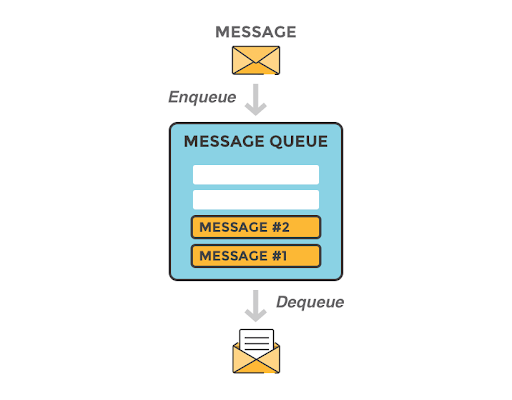
\includegraphics[width=0.8\textwidth]{Images/message.png}
			\centering
			\linebreak
			\caption{Active MQ}
	        \end{figure}
		        
            \textbf{Kiến trúc cơ bản}
            
            \begin{itemize}
                \item Message: Là thông tin cần gửi đi
                \item Producer: Là thành phần sẽ gửi message
                \item Consumer: Là thành phần nhận message
                \item Message Queue: Nơi chứa message, cho phép producer và consumer có thể trao đổi với nhau.
            \end{itemize}
            
            \textbf{Phân loại}
            
            \begin{itemize}
                \item Point-to-point: Tức là message chỉ được consume bởi 1 thành phần duy nhất
                
                \begin{figure}[H]   			
                	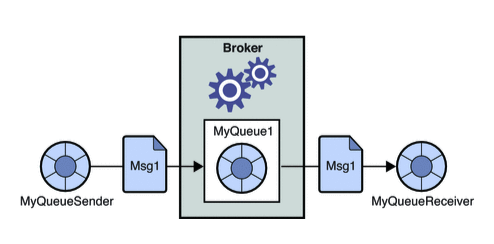
\includegraphics[width=0.8\textwidth]{Images/PTP.png}
	        		\centering
	        		\linebreak
	        		\caption{Point-to-point}
                \end{figure}
                
                \item Publisher-Subcriber: Ở đây ta có thể có nhiều consumer cùng consume 1 message giống nhau khi chúng cùng subcriber vào 1 topic.
                
                \begin{figure}[H]   			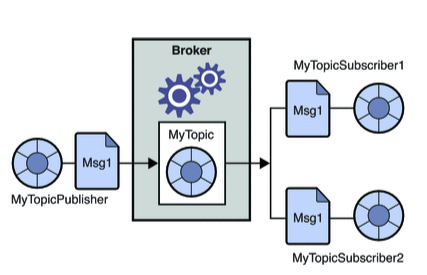
\includegraphics[width=0.8\textwidth]{Images/PS.png}
        		\centering
        		\linebreak
        		\caption{Publisher-Subcriber}
                \end{figure}
                
            \end{itemize}
            
            \textbf{Ưu điểm}
            
            \begin{itemize}
                \item Đảm bảo 1 message chỉ được xử lý đúng 1 lần duy nhất: Mỗi khi consumer lấy được message thì nó sẽ gửi 1 ACK về cho Broker, sau khi nhận được tín hiệu ACK thì Broker sẽ tiến hành xóa message đó đi để tránh việc 1 message được xử lý 2 lần.
                \item Nhắn tin không đồng bộ: Phù hợp với những việc không cần phải xử lý ngay lập tức. Lúc đó ta cứ đưa message vào queue rồi đi xử lý các công việc tiếp theo. Nhằm giảm response time đối với client.
                \item Tăng khả năng sẵn sàng: Giả sử ta có 2 service và lúc đó 1 trong 2 service đang trong trạng thái không hoạt động. Thì lúc đó hệ thống vẫn có thể hoạt động bình thường. Ta giữ các message trong queue đến khi service hoạt động lại thì nó consume message và tiếp tục công việc xử lý của nó
                \item Dễ dàng mở rộng: Mỗi khi lượng request tăng cao. Producer bắn message nhanh hơn tốc độ xử lý cả consumer thì lúc này ta chỉ đơn giản là thêm consumer vào để tăng tốc độ xử lý. Chú ý: Lúc này ta cần set tất cả các consumer chung 1 group-id để tránh việc 1 message có thể được xử lý nhiều lần.
            \end{itemize}
            
            \textbf{Nhược điểm}
            
            \begin{itemize}
                \item Làm phức tạp hệ thống: Khi thêm 1 thành phần thì ta phải chấp nhận việc xử lý phức tạp và có thể xảy ra sai sót trong quá trình xử lý.
                \item Producer và Consumer phải thống nhất về format của message: Mặc dù cả producer và consumer không quan tâm đến nhau (chỉ cần gửi message vào queue rồi thằng kia tới lấy) nhưng cả 2 cần có chung 1 format message để có thể dễ dàng xử lý sau khi consume.
                \item Monitor Queue: Ta cần phải theo dõi queue để biết được tình trạng hiện tại, queue có đầy hay không, có bị crash không để đưa ra phương án xử lý.
            \end{itemize}
            
            \textbf{Kết luận}\\
            
            Mặc dù message queue rất phù hợp để giao tiếp giữa các service trong hệ thống microservice. Nhưng ở đây nhóm chỉ sử dụng message để hiện thực cơ chế bất đồng bộ khi xử lý request tại một service cụ thế. Ví dụ như: Sau khi xử lý request của client ta cần vào Database để cập nhật lại status của đơn hàng nhưng việc truy xuất vào Database ngay thời điểm đó là không cần thiết. Ta có thể đưa message vào queue và sau đó trả kết quả về cho client ngay lập tức. Điều đó giúp ta tránh được việc truy xuất Database quá lâu sẽ ảnh hưởng đến trải nghiệm của người dùng.
            
            \subsection{Kafka}
            
            Kafka là dự án mã nguồn mở, đã được đóng gói hoàn chỉnh, khả năng chịu lỗi cao và là hệ thống nhắn tin nhanh. Vì tính đáng tin cậy của nó, kafka đang dần được thay thế cho hệ thống nhắn tin truyền thống. Nó được sử dụng cho các hệ thống nhắn tin thông thường trong các ngữ cảnh khác nhau. Đây là hệ quả khi khả năng mở rộng ngang và chuyển giao dữ liệu đáng tin cậy là những yêu cầu quan trọng nhất.\\
            
            Để có thể hiểu rõ vai trò của Kafka ta có thể xem ảnh sau
            
            \begin{figure}[H]   			
            	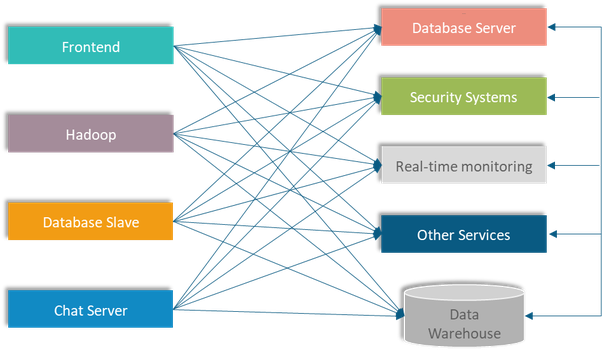
\includegraphics[width=0.8\textwidth]{Images/Kafka1.png}
    			\centering
    			\linebreak
    			\caption{Vai trò Kafka}
            \end{figure}
            
            Thông thường việc giao tiếp giữa các thành phần trong hệ thống diễn ra hết sức phức tạp. Điều này làm tăng chi phí giám sát và làm giảm hiệu suất của hệ thống.\\
            
            Và từ đó Kafka ra đời giúp chúng ta đơn giản đi việc giao tiếp giữa các thành phần trong hệ thống với nhau.
            
             \begin{figure}[H]   			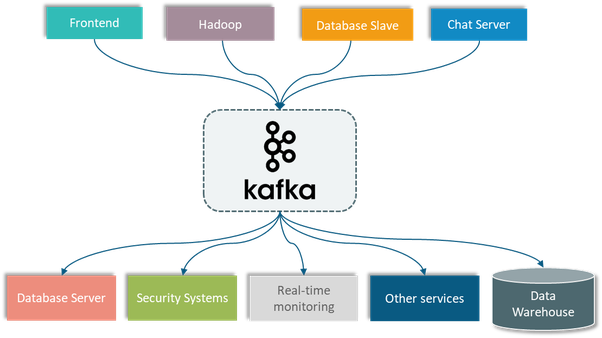
\includegraphics[width=0.8\textwidth]{Images/Kafka3.png}
    		\centering
    		\linebreak
    		\caption{Communicate giữa các hệ thống}
            \end{figure}
            
            \textbf{Kiến trúc}
            
             \begin{figure}[H]   			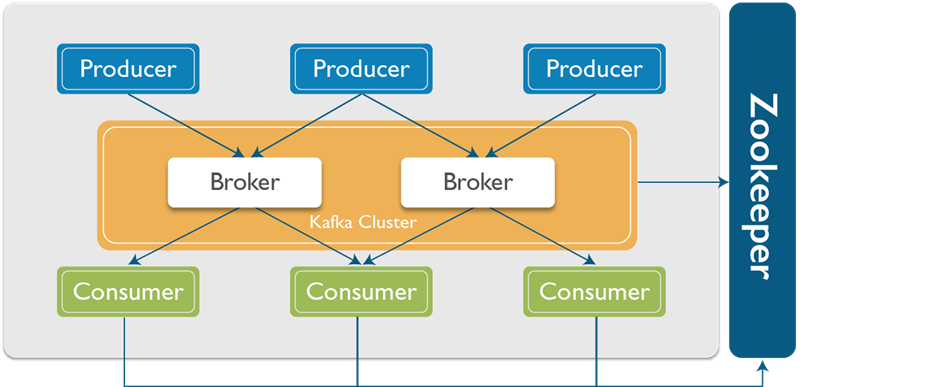
\includegraphics[width=0.8\textwidth]{Images/Kafka2.png}
    		\centering
    		\linebreak
    		\caption{Cấu trúc Kafka}
            \end{figure}
            
            \begin{itemize}
                \item Producer: Thành phần gửi message
                \item Message: Là message cần trao đổi đến các thành phần khác nhau trong hệ thống.
                \item Broker: Là tập hợp các server Kafka để lưu trữ các message
                \item Zookeeper: Được dùng để quản lý và bố trí các Broker
            \end{itemize}
            
    
          	\textbf{Kết luận}: Tại sao lại sử dụng Kafka và không sử dụng Message Queue truyền thống? \\
            
            Như nhóm đã trình bày ở phần trước thì Message Queue truyền thống sẽ đảm nhận nhiệm vụ xử lý bất đồng bộ trong từng service. Còn kafka sẽ là thành phần trung gian để gửi message từ service này đến service khác. Bởi vì kafka hoạt động rất nhanh do nó sử dụng cơ chế ZeroCopy, dữ liệu được sắp xếp theo khối, nén dữ liệu và giảm độ trễ I/O. Ngoài ra kafka rất dễ mở rộng khi lượng message cần trao đổi tăng lên và có cơ chế sao chép message ra nhiều partition để làm giảm rủi ro mất mát message trong quá trình xử lý.
            
            \subsection{Docker}
            
            Docker là nền tảng cung cấp cho các công cụ, service để các lập trình viên, quản lý hệ thống có thể phát triển, thực thi, chạy các ứng dụng với containers. Hay nói một cách khác nó là một nền tảng để cung cấp cách để building, deploy và run các ứng dụng một cách dễ dàng trên nền tảng ảo hóa - \textbf{"Build once, run anywhere"}. Hay nói một cách dễ hiểu như sau: Khi chúng ta muốn chạy app thì chúng ta phải thiết lập môi trường chạy cho nó. Thay vì chúng ta sẽ đi cài môi trường chạy cho nó thì chúng ta sẽ chạy docker.\\
            
            Ứng dụng Docker chạy trong vùng chứa (container) có thể được sử dụng trên bất kỳ hệ thống nào: máy tính xách tay của nhà phát triển, hệ thống trên cơ sở hoặc trong hệ thống đám mây. Và là một công cụ tạo môi trường được "đóng gói" (còn gọi là Container) trên máy tính mà không làm tác động tới môi trường hiện tại của máy, môi trường trong Docker sẽ chạy độc lập.\\
            
            Do nhóm viết ứng dụng theo kiến trúc Microservice vì thế có rất nhiều cơ sở hạ tầng phải deploy như: Cassandra, Kafka, Redis, Mysql, ActiveMQ, ... Ngoài ra còn rất nhiều service mà nhóm đã viết. Cho nên việc deploy và quản lý trên server vật lý hay virtual machine đều gặp rất nhiều khó khăn. Vì thế nhóm đã tìm hiểu và sử dụng Docker để đơn giản hóa quá trình deploy cơ sở hạ tầng và quản lý tài nguyên của mỗi service sao cho hiệu quả và tiết kiệm nhất. Đặc biệt việc sử dụng \textbf{Docker Compose} giúp chúng ta khởi tạo và quản lý các containers rất dễ dàng chi thông qua 1 dòng lệnh
            
			 \begin{figure}[H]
            	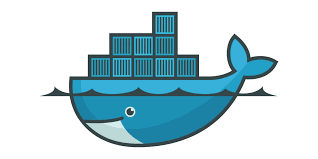
\includegraphics[width=0.8\textwidth]{Images/docker.png}
            	\centering
            	\linebreak
            	\caption{Giới thiệu về Docker}
            \end{figure}
            
            
            \subsection{NGINX}
            
            NGINX là một web server mạnh mẽ và sử dụng kiến trúc đơn luồng, hướng sự kiện vì thế nó hiệu quả hơn Apache server nếu được cấu hình chính xác. Nó cũng có thể làm những thứ quan trọng khác, chẳng hạn như load balancing, HTTP caching, hay sử dụng như một reverse proxy.\\
            
            NGINX được xây dựng để cung cấp việc sử dụng bộ nhớ thấp và đồng thời cao. Thay vì tạo các quy trình mới cho mỗi yêu cầu web, NGINX sử dụng cách tiếp cận theo hướng sự kiện, không đồng bộ trong đó các yêu cầu được xử lý trong một luồng.\\
            
            Reverse proxy là một proxy server mà khi đứng trước client, chúng hoạt động giống như những server bình thường. Reverse proxy chuyển tiếp request đến một hoặc nhiều server thật, kết quả sau đó trả về cho client như thể là chúng được trả về từ reverse proxy, khiến cho client không biết về những server thật nói trên. Reverse proxy được cài đặt trong một private network của một hoặc nhiều server, và tất cả lưu lượng truy cập đều phải đi qua proxy này.\\
            
            Nhờ vào reverse proxy nhóm có thể:
            
            \begin{itemize}
                \item Che giấu được thông tin các service được deploy bên trong private network.
                \item Tăng khả năng xử lý nhiều request dống thời.
                \item Phân chia tải cho các service bên trong.
                \item Thiêt lập cấu hình HTTPS.
            \end{itemize}
        
	        \begin{figure}[H]  			
	        	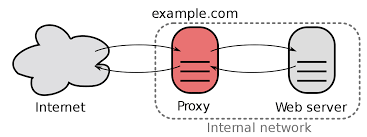
\includegraphics[width=0.8\textwidth]{Images/reverseproxy.png}
	        	\centering
	        	\linebreak
	        	\caption{Reverse Proxy}
	        \end{figure}
          
            
            
            
            
            
		